\normalfalse \difficiletrue \tdifficilefalse
\correctionfalse

%\UPSTIidClasse{11} % 11 sup, 12 spé
%\newcommand{\UPSTIidClasse}{12}

\exer{Poussoir $\star\star$ \label{B2:12:16}}
\setcounter{question}{0}\UPSTIcompetence{B2-12}
\index{Compétence B2-12}
%\index{Barrière Sympact}
\ifcorrection
\else
\marginnote{\textbf{Pas de corrigé pour cet exercice.}}
\fi

\ifprof
\else
\begin{center}
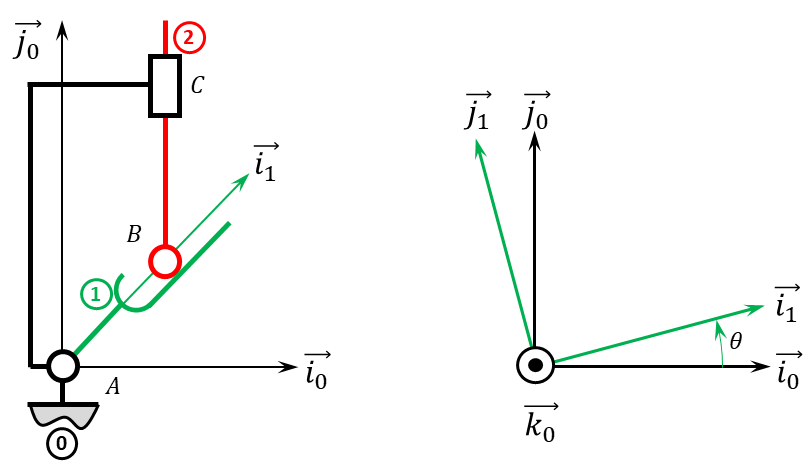
\includegraphics[width=\linewidth]{16_01}
\end{center}
\fi


\question{Réaliser le paramétrage du mécanisme.}
\ifprof
\else
\fi



\ifprof
\else
\begin{flushright}
\footnotesize{Corrigé  voir \ref{B2:12:16}.}
\end{flushright}%
\fi